\documentclass[12pt, a4paper, landscape]{memoir}
\usepackage[margin=0pt]{geometry}
\usepackage[utf8]{inputenc}
\usepackage{babel}
\usepackage[T1]{fontenc}
\usepackage{adjustbox}
\usepackage{amsmath}

\usepackage{tikz}
\usepackage{url}
\graphicspath{ {./images/} }

\pagenumbering{gobble}

\begin{document}
	\vspace*{-0.8em}
	\begin{center}
		{\LARGE Pascalov trojuholník}\\[1em]
		\large
		\begin{vplace}[0.5]
		\begin{adjustbox}{max width=.95\paperwidth, max height=.95\paperheight}	
			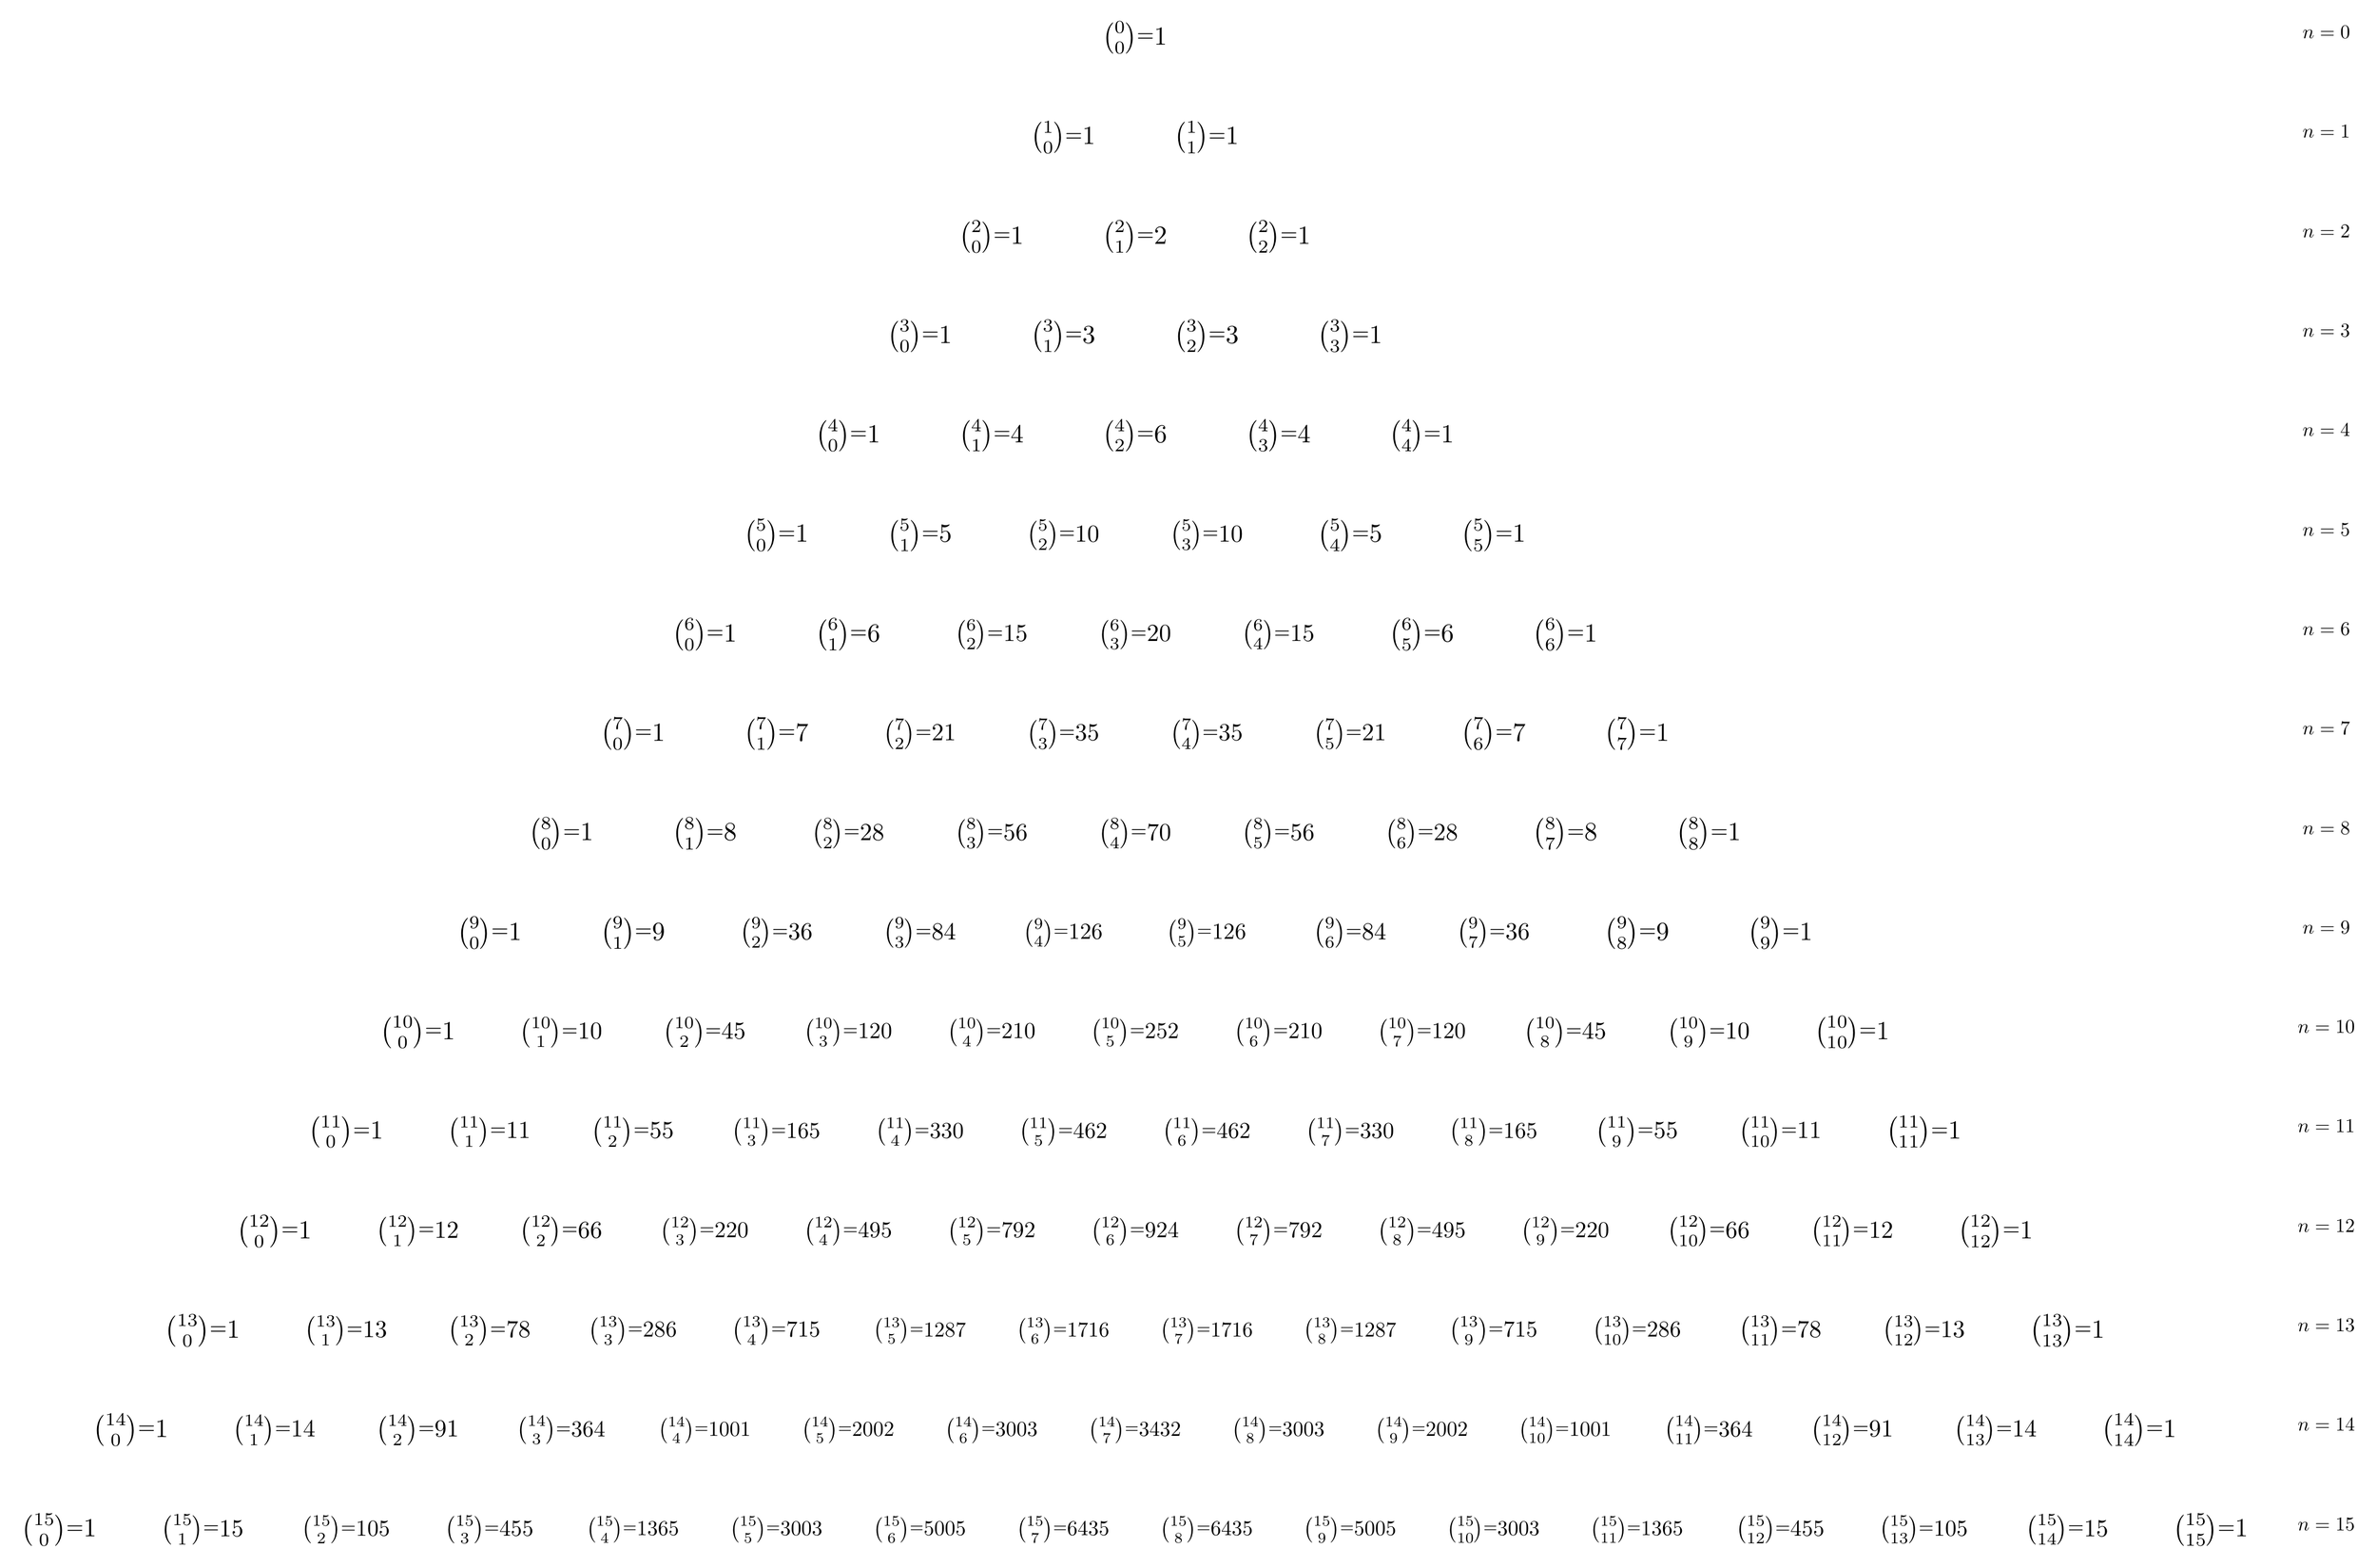
\begin{tikzpicture}
				\node[anchor=center] at (0.0, 0.0) {\scalebox{1.5999999999999999}{$\binom{0}{0}${\raisebox{.3ex}{\footnotesize=}$1$}}};
\node[anchor=center] at (25.75, 0.12) {\scalebox{1.2}{$n = 0$}};
\node[anchor=center] at (-1.55, -2.15) {\scalebox{1.5999999999999999}{$\binom{1}{0}${\raisebox{.3ex}{\footnotesize=}$1$}}};
\node[anchor=center] at (1.55, -2.15) {\scalebox{1.5999999999999999}{$\binom{1}{1}${\raisebox{.3ex}{\footnotesize=}$1$}}};
\node[anchor=center] at (25.75, -2.03) {\scalebox{1.2}{$n = 1$}};
\node[anchor=center] at (-3.1, -4.3) {\scalebox{1.5999999999999999}{$\binom{2}{0}${\raisebox{.3ex}{\footnotesize=}$1$}}};
\node[anchor=center] at (0.0, -4.3) {\scalebox{1.5999999999999999}{$\binom{2}{1}${\raisebox{.3ex}{\footnotesize=}$2$}}};
\node[anchor=center] at (3.1, -4.3) {\scalebox{1.5999999999999999}{$\binom{2}{2}${\raisebox{.3ex}{\footnotesize=}$1$}}};
\node[anchor=center] at (25.75, -4.18) {\scalebox{1.2}{$n = 2$}};
\node[anchor=center] at (-4.65, -6.449999999999999) {\scalebox{1.5999999999999999}{$\binom{3}{0}${\raisebox{.3ex}{\footnotesize=}$1$}}};
\node[anchor=center] at (-1.55, -6.449999999999999) {\scalebox{1.5999999999999999}{$\binom{3}{1}${\raisebox{.3ex}{\footnotesize=}$3$}}};
\node[anchor=center] at (1.55, -6.449999999999999) {\scalebox{1.5999999999999999}{$\binom{3}{2}${\raisebox{.3ex}{\footnotesize=}$3$}}};
\node[anchor=center] at (4.65, -6.449999999999999) {\scalebox{1.5999999999999999}{$\binom{3}{3}${\raisebox{.3ex}{\footnotesize=}$1$}}};
\node[anchor=center] at (25.75, -6.329999999999999) {\scalebox{1.2}{$n = 3$}};
\node[anchor=center] at (-6.2, -8.6) {\scalebox{1.5999999999999999}{$\binom{4}{0}${\raisebox{.3ex}{\footnotesize=}$1$}}};
\node[anchor=center] at (-3.1, -8.6) {\scalebox{1.5999999999999999}{$\binom{4}{1}${\raisebox{.3ex}{\footnotesize=}$4$}}};
\node[anchor=center] at (0.0, -8.6) {\scalebox{1.5999999999999999}{$\binom{4}{2}${\raisebox{.3ex}{\footnotesize=}$6$}}};
\node[anchor=center] at (3.1, -8.6) {\scalebox{1.5999999999999999}{$\binom{4}{3}${\raisebox{.3ex}{\footnotesize=}$4$}}};
\node[anchor=center] at (6.2, -8.6) {\scalebox{1.5999999999999999}{$\binom{4}{4}${\raisebox{.3ex}{\footnotesize=}$1$}}};
\node[anchor=center] at (25.75, -8.48) {\scalebox{1.2}{$n = 4$}};
\node[anchor=center] at (-7.75, -10.75) {\scalebox{1.5999999999999999}{$\binom{5}{0}${\raisebox{.3ex}{\footnotesize=}$1$}}};
\node[anchor=center] at (-4.65, -10.75) {\scalebox{1.5999999999999999}{$\binom{5}{1}${\raisebox{.3ex}{\footnotesize=}$5$}}};
\node[anchor=center] at (-1.55, -10.75) {\scalebox{1.5}{$\binom{5}{2}${\raisebox{.3ex}{\footnotesize=}$10$}}};
\node[anchor=center] at (1.55, -10.75) {\scalebox{1.5}{$\binom{5}{3}${\raisebox{.3ex}{\footnotesize=}$10$}}};
\node[anchor=center] at (4.65, -10.75) {\scalebox{1.5999999999999999}{$\binom{5}{4}${\raisebox{.3ex}{\footnotesize=}$5$}}};
\node[anchor=center] at (7.75, -10.75) {\scalebox{1.5999999999999999}{$\binom{5}{5}${\raisebox{.3ex}{\footnotesize=}$1$}}};
\node[anchor=center] at (25.75, -10.63) {\scalebox{1.2}{$n = 5$}};
\node[anchor=center] at (-9.3, -12.899999999999999) {\scalebox{1.5999999999999999}{$\binom{6}{0}${\raisebox{.3ex}{\footnotesize=}$1$}}};
\node[anchor=center] at (-6.2, -12.899999999999999) {\scalebox{1.5999999999999999}{$\binom{6}{1}${\raisebox{.3ex}{\footnotesize=}$6$}}};
\node[anchor=center] at (-3.1, -12.899999999999999) {\scalebox{1.5}{$\binom{6}{2}${\raisebox{.3ex}{\footnotesize=}$15$}}};
\node[anchor=center] at (0.0, -12.899999999999999) {\scalebox{1.5}{$\binom{6}{3}${\raisebox{.3ex}{\footnotesize=}$20$}}};
\node[anchor=center] at (3.1, -12.899999999999999) {\scalebox{1.5}{$\binom{6}{4}${\raisebox{.3ex}{\footnotesize=}$15$}}};
\node[anchor=center] at (6.2, -12.899999999999999) {\scalebox{1.5999999999999999}{$\binom{6}{5}${\raisebox{.3ex}{\footnotesize=}$6$}}};
\node[anchor=center] at (9.3, -12.899999999999999) {\scalebox{1.5999999999999999}{$\binom{6}{6}${\raisebox{.3ex}{\footnotesize=}$1$}}};
\node[anchor=center] at (25.75, -12.78) {\scalebox{1.2}{$n = 6$}};
\node[anchor=center] at (-10.85, -15.049999999999999) {\scalebox{1.5999999999999999}{$\binom{7}{0}${\raisebox{.3ex}{\footnotesize=}$1$}}};
\node[anchor=center] at (-7.75, -15.049999999999999) {\scalebox{1.5999999999999999}{$\binom{7}{1}${\raisebox{.3ex}{\footnotesize=}$7$}}};
\node[anchor=center] at (-4.65, -15.049999999999999) {\scalebox{1.5}{$\binom{7}{2}${\raisebox{.3ex}{\footnotesize=}$21$}}};
\node[anchor=center] at (-1.55, -15.049999999999999) {\scalebox{1.5}{$\binom{7}{3}${\raisebox{.3ex}{\footnotesize=}$35$}}};
\node[anchor=center] at (1.55, -15.049999999999999) {\scalebox{1.5}{$\binom{7}{4}${\raisebox{.3ex}{\footnotesize=}$35$}}};
\node[anchor=center] at (4.65, -15.049999999999999) {\scalebox{1.5}{$\binom{7}{5}${\raisebox{.3ex}{\footnotesize=}$21$}}};
\node[anchor=center] at (7.75, -15.049999999999999) {\scalebox{1.5999999999999999}{$\binom{7}{6}${\raisebox{.3ex}{\footnotesize=}$7$}}};
\node[anchor=center] at (10.85, -15.049999999999999) {\scalebox{1.5999999999999999}{$\binom{7}{7}${\raisebox{.3ex}{\footnotesize=}$1$}}};
\node[anchor=center] at (25.75, -14.93) {\scalebox{1.2}{$n = 7$}};
\node[anchor=center] at (-12.4, -17.2) {\scalebox{1.5999999999999999}{$\binom{8}{0}${\raisebox{.3ex}{\footnotesize=}$1$}}};
\node[anchor=center] at (-9.3, -17.2) {\scalebox{1.5999999999999999}{$\binom{8}{1}${\raisebox{.3ex}{\footnotesize=}$8$}}};
\node[anchor=center] at (-6.2, -17.2) {\scalebox{1.5}{$\binom{8}{2}${\raisebox{.3ex}{\footnotesize=}$28$}}};
\node[anchor=center] at (-3.1, -17.2) {\scalebox{1.5}{$\binom{8}{3}${\raisebox{.3ex}{\footnotesize=}$56$}}};
\node[anchor=center] at (0.0, -17.2) {\scalebox{1.5}{$\binom{8}{4}${\raisebox{.3ex}{\footnotesize=}$70$}}};
\node[anchor=center] at (3.1, -17.2) {\scalebox{1.5}{$\binom{8}{5}${\raisebox{.3ex}{\footnotesize=}$56$}}};
\node[anchor=center] at (6.2, -17.2) {\scalebox{1.5}{$\binom{8}{6}${\raisebox{.3ex}{\footnotesize=}$28$}}};
\node[anchor=center] at (9.3, -17.2) {\scalebox{1.5999999999999999}{$\binom{8}{7}${\raisebox{.3ex}{\footnotesize=}$8$}}};
\node[anchor=center] at (12.4, -17.2) {\scalebox{1.5999999999999999}{$\binom{8}{8}${\raisebox{.3ex}{\footnotesize=}$1$}}};
\node[anchor=center] at (25.75, -17.08) {\scalebox{1.2}{$n = 8$}};
\node[anchor=center] at (-13.950000000000001, -19.349999999999998) {\scalebox{1.5999999999999999}{$\binom{9}{0}${\raisebox{.3ex}{\footnotesize=}$1$}}};
\node[anchor=center] at (-10.85, -19.349999999999998) {\scalebox{1.5999999999999999}{$\binom{9}{1}${\raisebox{.3ex}{\footnotesize=}$9$}}};
\node[anchor=center] at (-7.75, -19.349999999999998) {\scalebox{1.5}{$\binom{9}{2}${\raisebox{.3ex}{\footnotesize=}$36$}}};
\node[anchor=center] at (-4.65, -19.349999999999998) {\scalebox{1.5}{$\binom{9}{3}${\raisebox{.3ex}{\footnotesize=}$84$}}};
\node[anchor=center] at (-1.55, -19.349999999999998) {\scalebox{1.4}{$\binom{9}{4}${\raisebox{.3ex}{\footnotesize=}$126$}}};
\node[anchor=center] at (1.55, -19.349999999999998) {\scalebox{1.4}{$\binom{9}{5}${\raisebox{.3ex}{\footnotesize=}$126$}}};
\node[anchor=center] at (4.65, -19.349999999999998) {\scalebox{1.5}{$\binom{9}{6}${\raisebox{.3ex}{\footnotesize=}$84$}}};
\node[anchor=center] at (7.75, -19.349999999999998) {\scalebox{1.5}{$\binom{9}{7}${\raisebox{.3ex}{\footnotesize=}$36$}}};
\node[anchor=center] at (10.85, -19.349999999999998) {\scalebox{1.5999999999999999}{$\binom{9}{8}${\raisebox{.3ex}{\footnotesize=}$9$}}};
\node[anchor=center] at (13.950000000000001, -19.349999999999998) {\scalebox{1.5999999999999999}{$\binom{9}{9}${\raisebox{.3ex}{\footnotesize=}$1$}}};
\node[anchor=center] at (25.75, -19.229999999999997) {\scalebox{1.2}{$n = 9$}};
\node[anchor=center] at (-15.5, -21.5) {\scalebox{1.5999999999999999}{$\binom{10}{0}${\raisebox{.3ex}{\footnotesize=}$1$}}};
\node[anchor=center] at (-12.4, -21.5) {\scalebox{1.5}{$\binom{10}{1}${\raisebox{.3ex}{\footnotesize=}$10$}}};
\node[anchor=center] at (-9.3, -21.5) {\scalebox{1.5}{$\binom{10}{2}${\raisebox{.3ex}{\footnotesize=}$45$}}};
\node[anchor=center] at (-6.2, -21.5) {\scalebox{1.4}{$\binom{10}{3}${\raisebox{.3ex}{\footnotesize=}$120$}}};
\node[anchor=center] at (-3.1, -21.5) {\scalebox{1.4}{$\binom{10}{4}${\raisebox{.3ex}{\footnotesize=}$210$}}};
\node[anchor=center] at (0.0, -21.5) {\scalebox{1.4}{$\binom{10}{5}${\raisebox{.3ex}{\footnotesize=}$252$}}};
\node[anchor=center] at (3.1, -21.5) {\scalebox{1.4}{$\binom{10}{6}${\raisebox{.3ex}{\footnotesize=}$210$}}};
\node[anchor=center] at (6.2, -21.5) {\scalebox{1.4}{$\binom{10}{7}${\raisebox{.3ex}{\footnotesize=}$120$}}};
\node[anchor=center] at (9.3, -21.5) {\scalebox{1.5}{$\binom{10}{8}${\raisebox{.3ex}{\footnotesize=}$45$}}};
\node[anchor=center] at (12.4, -21.5) {\scalebox{1.5}{$\binom{10}{9}${\raisebox{.3ex}{\footnotesize=}$10$}}};
\node[anchor=center] at (15.5, -21.5) {\scalebox{1.5999999999999999}{$\binom{10}{10}${\raisebox{.3ex}{\footnotesize=}$1$}}};
\node[anchor=center] at (25.75, -21.38) {\scalebox{1.2}{$n = 10$}};
\node[anchor=center] at (-17.05, -23.65) {\scalebox{1.5999999999999999}{$\binom{11}{0}${\raisebox{.3ex}{\footnotesize=}$1$}}};
\node[anchor=center] at (-13.950000000000001, -23.65) {\scalebox{1.5}{$\binom{11}{1}${\raisebox{.3ex}{\footnotesize=}$11$}}};
\node[anchor=center] at (-10.85, -23.65) {\scalebox{1.5}{$\binom{11}{2}${\raisebox{.3ex}{\footnotesize=}$55$}}};
\node[anchor=center] at (-7.75, -23.65) {\scalebox{1.4}{$\binom{11}{3}${\raisebox{.3ex}{\footnotesize=}$165$}}};
\node[anchor=center] at (-4.65, -23.65) {\scalebox{1.4}{$\binom{11}{4}${\raisebox{.3ex}{\footnotesize=}$330$}}};
\node[anchor=center] at (-1.55, -23.65) {\scalebox{1.4}{$\binom{11}{5}${\raisebox{.3ex}{\footnotesize=}$462$}}};
\node[anchor=center] at (1.55, -23.65) {\scalebox{1.4}{$\binom{11}{6}${\raisebox{.3ex}{\footnotesize=}$462$}}};
\node[anchor=center] at (4.65, -23.65) {\scalebox{1.4}{$\binom{11}{7}${\raisebox{.3ex}{\footnotesize=}$330$}}};
\node[anchor=center] at (7.75, -23.65) {\scalebox{1.4}{$\binom{11}{8}${\raisebox{.3ex}{\footnotesize=}$165$}}};
\node[anchor=center] at (10.85, -23.65) {\scalebox{1.5}{$\binom{11}{9}${\raisebox{.3ex}{\footnotesize=}$55$}}};
\node[anchor=center] at (13.950000000000001, -23.65) {\scalebox{1.5}{$\binom{11}{10}${\raisebox{.3ex}{\footnotesize=}$11$}}};
\node[anchor=center] at (17.05, -23.65) {\scalebox{1.5999999999999999}{$\binom{11}{11}${\raisebox{.3ex}{\footnotesize=}$1$}}};
\node[anchor=center] at (25.75, -23.529999999999998) {\scalebox{1.2}{$n = 11$}};
\node[anchor=center] at (-18.6, -25.799999999999997) {\scalebox{1.5999999999999999}{$\binom{12}{0}${\raisebox{.3ex}{\footnotesize=}$1$}}};
\node[anchor=center] at (-15.5, -25.799999999999997) {\scalebox{1.5}{$\binom{12}{1}${\raisebox{.3ex}{\footnotesize=}$12$}}};
\node[anchor=center] at (-12.4, -25.799999999999997) {\scalebox{1.5}{$\binom{12}{2}${\raisebox{.3ex}{\footnotesize=}$66$}}};
\node[anchor=center] at (-9.3, -25.799999999999997) {\scalebox{1.4}{$\binom{12}{3}${\raisebox{.3ex}{\footnotesize=}$220$}}};
\node[anchor=center] at (-6.2, -25.799999999999997) {\scalebox{1.4}{$\binom{12}{4}${\raisebox{.3ex}{\footnotesize=}$495$}}};
\node[anchor=center] at (-3.1, -25.799999999999997) {\scalebox{1.4}{$\binom{12}{5}${\raisebox{.3ex}{\footnotesize=}$792$}}};
\node[anchor=center] at (0.0, -25.799999999999997) {\scalebox{1.4}{$\binom{12}{6}${\raisebox{.3ex}{\footnotesize=}$924$}}};
\node[anchor=center] at (3.1, -25.799999999999997) {\scalebox{1.4}{$\binom{12}{7}${\raisebox{.3ex}{\footnotesize=}$792$}}};
\node[anchor=center] at (6.2, -25.799999999999997) {\scalebox{1.4}{$\binom{12}{8}${\raisebox{.3ex}{\footnotesize=}$495$}}};
\node[anchor=center] at (9.3, -25.799999999999997) {\scalebox{1.4}{$\binom{12}{9}${\raisebox{.3ex}{\footnotesize=}$220$}}};
\node[anchor=center] at (12.4, -25.799999999999997) {\scalebox{1.5}{$\binom{12}{10}${\raisebox{.3ex}{\footnotesize=}$66$}}};
\node[anchor=center] at (15.5, -25.799999999999997) {\scalebox{1.5}{$\binom{12}{11}${\raisebox{.3ex}{\footnotesize=}$12$}}};
\node[anchor=center] at (18.6, -25.799999999999997) {\scalebox{1.5999999999999999}{$\binom{12}{12}${\raisebox{.3ex}{\footnotesize=}$1$}}};
\node[anchor=center] at (25.75, -25.679999999999996) {\scalebox{1.2}{$n = 12$}};
\node[anchor=center] at (-20.150000000000002, -27.95) {\scalebox{1.5999999999999999}{$\binom{13}{0}${\raisebox{.3ex}{\footnotesize=}$1$}}};
\node[anchor=center] at (-17.05, -27.95) {\scalebox{1.5}{$\binom{13}{1}${\raisebox{.3ex}{\footnotesize=}$13$}}};
\node[anchor=center] at (-13.950000000000001, -27.95) {\scalebox{1.5}{$\binom{13}{2}${\raisebox{.3ex}{\footnotesize=}$78$}}};
\node[anchor=center] at (-10.85, -27.95) {\scalebox{1.4}{$\binom{13}{3}${\raisebox{.3ex}{\footnotesize=}$286$}}};
\node[anchor=center] at (-7.75, -27.95) {\scalebox{1.4}{$\binom{13}{4}${\raisebox{.3ex}{\footnotesize=}$715$}}};
\node[anchor=center] at (-4.65, -27.95) {\scalebox{1.2999999999999998}{$\binom{13}{5}${\raisebox{.3ex}{\footnotesize=}$1287$}}};
\node[anchor=center] at (-1.55, -27.95) {\scalebox{1.2999999999999998}{$\binom{13}{6}${\raisebox{.3ex}{\footnotesize=}$1716$}}};
\node[anchor=center] at (1.55, -27.95) {\scalebox{1.2999999999999998}{$\binom{13}{7}${\raisebox{.3ex}{\footnotesize=}$1716$}}};
\node[anchor=center] at (4.65, -27.95) {\scalebox{1.2999999999999998}{$\binom{13}{8}${\raisebox{.3ex}{\footnotesize=}$1287$}}};
\node[anchor=center] at (7.75, -27.95) {\scalebox{1.4}{$\binom{13}{9}${\raisebox{.3ex}{\footnotesize=}$715$}}};
\node[anchor=center] at (10.85, -27.95) {\scalebox{1.4}{$\binom{13}{10}${\raisebox{.3ex}{\footnotesize=}$286$}}};
\node[anchor=center] at (13.950000000000001, -27.95) {\scalebox{1.5}{$\binom{13}{11}${\raisebox{.3ex}{\footnotesize=}$78$}}};
\node[anchor=center] at (17.05, -27.95) {\scalebox{1.5}{$\binom{13}{12}${\raisebox{.3ex}{\footnotesize=}$13$}}};
\node[anchor=center] at (20.150000000000002, -27.95) {\scalebox{1.5999999999999999}{$\binom{13}{13}${\raisebox{.3ex}{\footnotesize=}$1$}}};
\node[anchor=center] at (25.75, -27.83) {\scalebox{1.2}{$n = 13$}};
\node[anchor=center] at (-21.7, -30.099999999999998) {\scalebox{1.5999999999999999}{$\binom{14}{0}${\raisebox{.3ex}{\footnotesize=}$1$}}};
\node[anchor=center] at (-18.6, -30.099999999999998) {\scalebox{1.5}{$\binom{14}{1}${\raisebox{.3ex}{\footnotesize=}$14$}}};
\node[anchor=center] at (-15.5, -30.099999999999998) {\scalebox{1.5}{$\binom{14}{2}${\raisebox{.3ex}{\footnotesize=}$91$}}};
\node[anchor=center] at (-12.4, -30.099999999999998) {\scalebox{1.4}{$\binom{14}{3}${\raisebox{.3ex}{\footnotesize=}$364$}}};
\node[anchor=center] at (-9.3, -30.099999999999998) {\scalebox{1.2999999999999998}{$\binom{14}{4}${\raisebox{.3ex}{\footnotesize=}$1001$}}};
\node[anchor=center] at (-6.2, -30.099999999999998) {\scalebox{1.2999999999999998}{$\binom{14}{5}${\raisebox{.3ex}{\footnotesize=}$2002$}}};
\node[anchor=center] at (-3.1, -30.099999999999998) {\scalebox{1.2999999999999998}{$\binom{14}{6}${\raisebox{.3ex}{\footnotesize=}$3003$}}};
\node[anchor=center] at (0.0, -30.099999999999998) {\scalebox{1.2999999999999998}{$\binom{14}{7}${\raisebox{.3ex}{\footnotesize=}$3432$}}};
\node[anchor=center] at (3.1, -30.099999999999998) {\scalebox{1.2999999999999998}{$\binom{14}{8}${\raisebox{.3ex}{\footnotesize=}$3003$}}};
\node[anchor=center] at (6.2, -30.099999999999998) {\scalebox{1.2999999999999998}{$\binom{14}{9}${\raisebox{.3ex}{\footnotesize=}$2002$}}};
\node[anchor=center] at (9.3, -30.099999999999998) {\scalebox{1.2999999999999998}{$\binom{14}{10}${\raisebox{.3ex}{\footnotesize=}$1001$}}};
\node[anchor=center] at (12.4, -30.099999999999998) {\scalebox{1.4}{$\binom{14}{11}${\raisebox{.3ex}{\footnotesize=}$364$}}};
\node[anchor=center] at (15.5, -30.099999999999998) {\scalebox{1.5}{$\binom{14}{12}${\raisebox{.3ex}{\footnotesize=}$91$}}};
\node[anchor=center] at (18.6, -30.099999999999998) {\scalebox{1.5}{$\binom{14}{13}${\raisebox{.3ex}{\footnotesize=}$14$}}};
\node[anchor=center] at (21.7, -30.099999999999998) {\scalebox{1.5999999999999999}{$\binom{14}{14}${\raisebox{.3ex}{\footnotesize=}$1$}}};
\node[anchor=center] at (25.75, -29.979999999999997) {\scalebox{1.2}{$n = 14$}};
\node[anchor=center] at (-23.25, -32.25) {\scalebox{1.5999999999999999}{$\binom{15}{0}${\raisebox{.3ex}{\footnotesize=}$1$}}};
\node[anchor=center] at (-20.150000000000002, -32.25) {\scalebox{1.5}{$\binom{15}{1}${\raisebox{.3ex}{\footnotesize=}$15$}}};
\node[anchor=center] at (-17.05, -32.25) {\scalebox{1.4}{$\binom{15}{2}${\raisebox{.3ex}{\footnotesize=}$105$}}};
\node[anchor=center] at (-13.950000000000001, -32.25) {\scalebox{1.4}{$\binom{15}{3}${\raisebox{.3ex}{\footnotesize=}$455$}}};
\node[anchor=center] at (-10.85, -32.25) {\scalebox{1.2999999999999998}{$\binom{15}{4}${\raisebox{.3ex}{\footnotesize=}$1365$}}};
\node[anchor=center] at (-7.75, -32.25) {\scalebox{1.2999999999999998}{$\binom{15}{5}${\raisebox{.3ex}{\footnotesize=}$3003$}}};
\node[anchor=center] at (-4.65, -32.25) {\scalebox{1.2999999999999998}{$\binom{15}{6}${\raisebox{.3ex}{\footnotesize=}$5005$}}};
\node[anchor=center] at (-1.55, -32.25) {\scalebox{1.2999999999999998}{$\binom{15}{7}${\raisebox{.3ex}{\footnotesize=}$6435$}}};
\node[anchor=center] at (1.55, -32.25) {\scalebox{1.2999999999999998}{$\binom{15}{8}${\raisebox{.3ex}{\footnotesize=}$6435$}}};
\node[anchor=center] at (4.65, -32.25) {\scalebox{1.2999999999999998}{$\binom{15}{9}${\raisebox{.3ex}{\footnotesize=}$5005$}}};
\node[anchor=center] at (7.75, -32.25) {\scalebox{1.2999999999999998}{$\binom{15}{10}${\raisebox{.3ex}{\footnotesize=}$3003$}}};
\node[anchor=center] at (10.85, -32.25) {\scalebox{1.2999999999999998}{$\binom{15}{11}${\raisebox{.3ex}{\footnotesize=}$1365$}}};
\node[anchor=center] at (13.950000000000001, -32.25) {\scalebox{1.4}{$\binom{15}{12}${\raisebox{.3ex}{\footnotesize=}$455$}}};
\node[anchor=center] at (17.05, -32.25) {\scalebox{1.4}{$\binom{15}{13}${\raisebox{.3ex}{\footnotesize=}$105$}}};
\node[anchor=center] at (20.150000000000002, -32.25) {\scalebox{1.5}{$\binom{15}{14}${\raisebox{.3ex}{\footnotesize=}$15$}}};
\node[anchor=center] at (23.25, -32.25) {\scalebox{1.5999999999999999}{$\binom{15}{15}${\raisebox{.3ex}{\footnotesize=}$1$}}};
\node[anchor=center] at (25.75, -32.13) {\scalebox{1.2}{$n = 15$}};
			\end{tikzpicture}
		\end{adjustbox}
		\end{vplace}
	\end{center}
\end{document}
